\subsection{Unresolved edges, survivor invariant, and query retirement}
\label{app:lower-proof-invariant}

We need two facts under the instance--midpoint law
\eqref{app:eq:joint-instance-midpoint-law}:
\begin{itemize}
\item \emph{The distribution left unresolved.}
\Cref{app:lem:unresolved-invariant} shows that the remaining matching is
uniform and its triggers are independent uniform remaining candidates.
This permits the conditional collision calculation below.
\item \emph{The number of query retirements.}
\Cref{app:lem:query-disclosure} bounds
\(\mathbb E\GenieDeletions\le N\QueryBudget{}/\HardBankSize\).
A submission tests at most one candidate at each source, so probes can
retire only a limited number of edges before commits touch them.
\end{itemize}
We first define retirement and the information used to condition these
two statements. The decision-rule seed \(w\) remains fixed.
Use the operation clock, actions \(A_s\), and visible histories
\(\OpVisibleHistory{s}\) from
\cref{app:eq:operation-action,app:eq:operation-visible-history}.
For a query, write \(y=\OpSubmittedState{s}\) and \(J=J_s\).
At commit \(t\), \(s=s_t\) and the batch is \(B_t=B_{t_s}\).

\begin{definition*}[Unresolved edges and the analytic record]
\emph{The test at one source.}
For any submitted state \(y\) and position \(i\in\PositionSet\), put
\begin{equation}
 \HardTest{y}{i}:=
 \begin{cases}
  c,&y_i=\HardCandidate{c}\text{ for some }c\in[\HardBankSize],\\
  \bot,&y_i=\MASK\text{ or }y_i\in\HardBackground,
 \end{cases}
 \qquad
 \HardHit{y}{i}:=
 \mathbf 1\{\HardTest{y}{i}=\TriggerIndex{i}\}.
 \label{app:eq:hard-test-and-hit}
\end{equation}
Thus \(y_i=\HardCandidate{c}\) tests the equality
\(\TriggerIndex{i}=c\). A mask or background value tests no candidate.

\emph{Unresolved edges and vertices.}
Let \(\OpUnresolvedMatching{s}\) be the edges unresolved immediately
before operation \(s\). Initialize \(\OpUnresolvedMatching{1}:=\HiddenMatching\)
and update by
\begin{equation}
 \OpUnresolvedMatching{s+1}:=
 \begin{cases}
  \{e\in\OpUnresolvedMatching{s}:
       \sum_{i\in e}\HardHit{y}{i}=0\},
       &\text{query of }y,\\
  \{e\in\OpUnresolvedMatching{s}:e\cap B_t=\varnothing\},
       &\text{commit }t.
 \end{cases}
 \label{app:eq:unresolved-matching-update}
\end{equation}
Define the unresolved vertex set by
\begin{equation}
 \OpUnresolvedVertices{s}:=\bigcup_{e\in\OpUnresolvedMatching{s}}e.
 \label{app:eq:unresolved-vertices}
\end{equation}
Thus a query retires an edge when at least one endpoint hits; a commit
retires it when \(e\cap B_t\ne\varnothing\). In either case both endpoints
leave \(\OpUnresolvedVertices{s}\). A query commits neither endpoint,
and a commit fixes only those in \(e\cap B_t\).
Because each update removes whole edges, \(\OpUnresolvedMatching{s}\)
is a perfect matching on \(\OpUnresolvedVertices{s}\).
The target law remains
\(\HardTargetLaw{I}(x)=\prod_{e\in\HiddenMatching}\HardEdgeLaw{e}{I}(x_e)\),
and the frozen oracle \(\HardOracle{I}\) remains unchanged.
In particular, an uncommitted vertex may lie on a retired edge.

\emph{Retirement record.}
For each newly retired edge, record its identity and both trigger indices:
\begin{equation}
 \OpRetiredRecord{s}:=
 \left\{\bigl(e,(\TriggerIndex{i})_{i\in e}\bigr):
 e\in\OpUnresolvedMatching{s}\setminus\OpUnresolvedMatching{s+1}\right\}.
 \label{app:eq:retirement-record}
\end{equation}
Endpoint tuples use the public position order. Let
\(\GenieDeletions:=\sum_{s:\,A_s\text{ is a query}}
 |\OpUnresolvedMatching{s}\setminus\OpUnresolvedMatching{s+1}|\).
Simultaneous hits on both endpoints count as one retired edge.

\emph{Remaining candidates.}
Initially \(\OpRemainingTriggers{i}{1}:=[\HardBankSize]\).
For each surviving \(i\in\OpUnresolvedVertices{s+1}\), put
\begin{equation}
 \OpRemainingTriggers{i}{s+1}:=
 \begin{cases}
  \OpRemainingTriggers{i}{s}\setminus\{\HardTest{y}{i}\},
       &\text{query of }y,\\
  \OpRemainingTriggers{i}{s},&\text{commit}.
 \end{cases}
 \label{app:eq:operation-candidates}
\end{equation}
A surviving endpoint has hit bit zero, so any candidate tested there
has failed. Subtracting \(\bot\) or a previously excluded candidate
changes nothing. Candidate sets are needed only while the vertex survives.

\emph{Analytic observations and history.}
Use the ordinary observation \(\OpVisibleObservation{s}\) from
\cref{app:eq:operation-visible-observation}, with
\(\FrozenOracle=\HardOracle{I}\). At a commit,
\(z_s=X_{B_t}\) is drawn from the midpoint kernel
\(\HardMidpointKernel{t}{I}(\cdot\mid\OpVisibleHistory{s})\)
of \cref{app:eq:hard-midpoint-kernel}.
The additional information is:
\begin{itemize}
\item At a query, the entire hit-bit vector
\(\bigl(\HardHit{y}{i}\bigr)_{i\in\OpUnresolvedVertices{s}}\)
from \cref{app:eq:hard-test-and-hit}, including bits whose mate rows
were not requested. Evaluate these bits on the same pre-operation
set \(\OpUnresolvedVertices{s}\), then apply
\cref{app:eq:unresolved-matching-update}.
\item At each retirement, the tuples in \(\OpRetiredRecord{s}\) from
\cref{app:eq:retirement-record}. Commit values \(X_{B_t}\) are already
part of the ordinary observation, not additional hidden information.
\end{itemize}
Formally, initialize \(\OpAnalyticHistory{1}:=\OpVisibleHistory{1}\)
and define
\begin{equation}
 \OpObservation{s}:=
 \begin{cases}
  \bigl(\OpVisibleObservation{s},
       (\HardHit{y}{i})_{i\in\OpUnresolvedVertices{s}}\bigr),
       &\text{query of }y,\\
  \OpVisibleObservation{s},&\text{commit},
 \end{cases}
 \label{app:eq:analytic-observation}
\end{equation}
\begin{equation}
 \OpAnalyticHistory{(s+1)}
 :=(\OpAnalyticHistory{s},A_s,\OpObservation{s},\OpRetiredRecord{s}).
 \label{app:eq:analytic-record-update}
\end{equation}
The decision rule uses only the ordinary observations in
\cref{app:eq:operation-visible-history}; it does not receive hit bits
or retirement disclosures. Its internal state is recoverable from that
visible history. Define the analytic sigma-field and hidden survivor state by
\begin{equation}
 \begin{aligned}
 \OpAnalyticField{s}
   &:=\sigma(\OpAnalyticHistory{s},\OpUnresolvedVertices{s}),\\
 \OpSurvivorState{s}
   &:=\bigl(\OpUnresolvedMatching{s},
          (\TriggerIndex{i})_{i\in\OpUnresolvedVertices{s}}\bigr).
 \end{aligned}
 \label{app:eq:analytic-field-and-survivor}
\end{equation}
The visible history is a projection of the analytic record, so
\(\sigma(\OpVisibleHistory{s})\subseteq\OpAnalyticField{s}\).
The unresolved vertices are recoverable by removing all recorded retired
endpoints from \(\PositionSet\); their remaining matching and triggers
are not explicitly recorded. The survivor state \(\OpSurvivorState{s}\)
is not itself an entry of the record.
Here \emph{unresolved} means survival under
\cref{app:eq:unresolved-matching-update}, not a claim about the
algorithm's knowledge.
\end{definition*}

One state supplies at most one test per source, even if many returned rows
are inspected. Its submission contributes one to
\(\CounterfactualQueries\le\QueryBudget{}\), as in
\textcolor{red}{\cref{app:def:resources}}. A state inducing no tests still counts,
except for the separately accounted distinguished preprocessing readout.
Retired edges can still affect ordinary oracle replies; they are excluded
only from subsequent unresolved-edge collision counts.

\paragraph{State immediately before a commit.}
At operation \(s_t\), use the shorter pre-commit notation for the
objects in \cref{app:eq:unresolved-vertices,app:eq:operation-candidates,app:eq:analytic-record-update,app:eq:analytic-field-and-survivor}:
\begin{equation}
 \begin{aligned}
 \UnresolvedVertices{t}&:=\OpUnresolvedVertices{s_t},&
 \RemainingTriggers{i}{t}&:=\OpRemainingTriggers{i}{s_t},\\
 \AnalyticHistory{t}&:=\OpAnalyticHistory{s_t},&
 \AnalyticField{t}&:=\OpAnalyticField{s_t},\\
 \SurvivorState{t}&:=\OpSurvivorState{s_t},&
 H_{t-1}&=\OpVisibleHistory{s_t}.
 \end{aligned}
 \label{app:eq:remaining-trigger-set}
\end{equation}
Here \(H_{t-1}\) is the complete visible history used in
\cref{app:lem:adaptive-midpoint-lower}, after any queries preceding commit
\(t\). There may be queries before commit \(1\), so
\(\UnresolvedVertices{1}\) need not equal \(\PositionSet\).
The next operation after commit \(t\) is \(s_t+1\); intervening queries
are processed before the next commit boundary \(s_{t+1}\).

\paragraph{Why uniformity can survive an observation.}
A failed test removes one candidate. A hit or a commit instead retires
the affected edge and records both its triggers.
We show that, once this retired record is fixed, the probability of the
complete new observation is the same for every compatible remaining
matching and trigger assignment. Equal prior weights therefore give equal
posterior weights.

% Please keep the invariant statement together before starting its proof.
\Needspace{10\baselineskip}
\begin{lemma}[Unresolved-matching invariant]
\label{app:lem:unresolved-invariant}
Under the joint law \eqref{app:eq:joint-instance-midpoint-law},
\begin{equation}
 \SurvivorState{t}\mid\AnalyticField{t}
 \sim
 \operatorname{Unif}\bigl(\operatorname{PM}
   (\UnresolvedVertices{t})\bigr)
 \otimes
 \bigotimes_{i\in\UnresolvedVertices{t}}
 \operatorname{Unif}(\RemainingTriggers{i}{t}),
 \label{app:eq:strong-survivor-invariant}
\end{equation}
where \(\operatorname{PM}(U)\) denotes the perfect matchings of \(U\).
In particular, the unresolved matching is conditionally uniform, and every
surviving trigger is conditionally uniform on its untested candidates.
The same product law holds at every analytic operation boundary, with the
current unresolved set, remaining-candidate sets, and analytic sigma-field in
place of their pre-commit notation above.
\end{lemma}

{\color{blue}
\begin{proof}[Simplified proof via conditional independence]
We prove the operation-boundary statement and then specialize it to the
pre-commit boundaries.  We use the operation-time notation already defined
in \cref{app:eq:unresolved-vertices,app:eq:operation-candidates,app:eq:analytic-record-update,app:eq:analytic-field-and-survivor},
without introducing shorter names for these objects.  The desired induction
step has two parts:
\begin{enumerate}
\item after conditioning on the newly retired edges and their triggers,
the new survivor state still has the required product-uniform law; and
\item the new observation is conditionally independent of that survivor
state once the retirement record is fixed.
\end{enumerate}
Indeed, these two statements give
\begin{align*}
 &\mathcal L\!\left(
   \OpSurvivorState{s+1}\,\middle|\,
   \OpAnalyticField{s},\OpRetiredRecord{s},\OpObservation{s}\right)\\
 &\qquad=
 \mathcal L\!\left(
   \OpSurvivorState{s+1}\,\middle|\,
   \OpAnalyticField{s},\OpRetiredRecord{s}\right),
\end{align*}
and the conditioning field on the left is precisely
\(\OpAnalyticField{(s+1)}\), by
\cref{app:eq:analytic-record-update,app:eq:analytic-field-and-survivor}.

\emph{1. Initialize the induction.}
Before operation \(1\), the unresolved matching is uniform on
\(\operatorname{PM}(\PositionSet)\), and the trigger indices are mutually
independent and uniform on \([\HardBankSize]\), independently of the
matching.  Thus the required product law holds at the initial boundary.

Now assume that, conditionally on \(\OpAnalyticField{s}\),
\[
 \OpSurvivorState{s}
 \sim
 \operatorname{Unif}\bigl(
   \operatorname{PM}(\OpUnresolvedVertices{s})\bigr)
 \otimes
 \bigotimes_{i\in\OpUnresolvedVertices{s}}
 \operatorname{Unif}(\OpRemainingTriggers{i}{s}).
\]
The action \(A_s\) is already determined by \(\OpAnalyticField{s}\), because
the seed-fixed decision rule uses the visible history contained in this
field.

\emph{2. Condition first on the retirement record.}
Fix a retirement record of positive conditional probability,
\[
 \RetiredRecordValue
 =\{(e,(\theta_i^{\RetiredRecordValue})_{i\in e}):e\in E_0\},
 \qquad
 D_0:=\bigcup_{e\in E_0}e,
\]
where \(E_0\) is the set of edges retired in operation \(s\) and \(D_0\)
is its endpoint set.  On
\(\{\OpRetiredRecord{s}=\RetiredRecordValue\}\),
\[
 \OpUnresolvedVertices{s+1}
 =\OpUnresolvedVertices{s}\setminus D_0.
\]
For every \(i\in\OpUnresolvedVertices{s+1}\), the update already defined in
\eqref{app:eq:operation-candidates} reads
\[
 \OpRemainingTriggers{i}{s+1}=
 \begin{cases}
  \OpRemainingTriggers{i}{s}\setminus
       \{\HardTest{y}{i}\},&A_s\text{ is a query of }y,\\
  \OpRemainingTriggers{i}{s},&A_s\text{ is a commit}.
 \end{cases}
\]
For an edge \(e=\{i,j\}\in\OpUnresolvedMatching{s}\), the update
\eqref{app:eq:unresolved-matching-update} is equivalently
\[
 e\in\OpUnresolvedMatching{s+1}
 \quad\Longleftrightarrow\quad
 \begin{cases}
  \HardHit{y}{i}=\HardHit{y}{j}=0,
       &A_s\text{ is a query of }y,\\
  e\cap B_t=\varnothing,
       &A_s\text{ is commit }t.
 \end{cases}
\]
In the query case, a candidate \(\theta_i\) at a surviving endpoint obeys
\[
 \theta_i\in\OpRemainingTriggers{i}{s+1}
 \quad\Longleftrightarrow\quad
 \theta_i\in\OpRemainingTriggers{i}{s}
 \ \text{and}\
 \theta_i\ne\HardTest{y}{i}.
\]
This also covers \(\HardTest{y}{i}=\bot\), because trigger indices lie in
\([\HardBankSize]\).  Since the fixed record has positive conditional
probability, each \(e\in E_0\) satisfies the complementary retirement
condition: at least one endpoint hits in the query case, and
\(e\cap B_t\ne\varnothing\) in the commit case.
Hence the complete support of the new survivor state, after fixing
\(\RetiredRecordValue\), is
\[
 \operatorname{PM}(\OpUnresolvedVertices{s+1})
 \times
 \prod_{i\in\OpUnresolvedVertices{s+1}}
       \OpRemainingTriggers{i}{s+1}.
\]

We now verify explicitly that every element of this Cartesian support has
the same conditional weight.  Fix
\(
 \SurvivorConfigA
 =\left(M',(\theta_i)_{i\in\OpUnresolvedVertices{s+1}}\right)
 \in
 \operatorname{PM}(\OpUnresolvedVertices{s+1})
 \times
 \prod_{i\in\OpUnresolvedVertices{s+1}}
       \OpRemainingTriggers{i}{s+1}
\).
Together, \(\SurvivorConfigA\) and \(\RetiredRecordValue\) reconstruct exactly one
pre-operation state: its unresolved matching is
\(M'\mathbin{\dot\cup}E_0\), its trigger is \(\theta_i\) on
\(\OpUnresolvedVertices{s+1}\), and its trigger is
\(\theta_i^{\RetiredRecordValue}\) on \(D_0\).  Conversely, membership in the
displayed support ensures that this reconstructed state produces the fixed
retirement record.  Since
\[
 \OpUnresolvedVertices{s}
 =\OpUnresolvedVertices{s+1}\mathbin{\dot\cup}D_0,
\]
these two constructions are inverse to each other.  The induction hypothesis
therefore gives the same joint mass to every compatible
\(\SurvivorConfigA\):
\[
\begin{aligned}
 &\mathbb P\!\left(
   \OpSurvivorState{s+1}=\SurvivorConfigA,\,
   \OpRetiredRecord{s}=\RetiredRecordValue
   \,\middle|\,\OpAnalyticField{s}\right)\\
 &\quad=
 \mathbb P\!\left(
 \begin{gathered}
  \OpUnresolvedMatching{s}=M'\mathbin{\dot\cup}E_0,\\
  \TriggerIndex{i}=\theta_i
       \quad(i\in\OpUnresolvedVertices{s+1}),\\
  \TriggerIndex{i}=\theta_i^{\RetiredRecordValue}\quad(i\in D_0)
 \end{gathered}
 \middle|\OpAnalyticField{s}\right)\\
 &\quad=
 \underbrace{
 \frac{1}{|\operatorname{PM}(\OpUnresolvedVertices{s})|}
 \prod_{i\in\OpUnresolvedVertices{s}}
       \frac{1}{|\OpRemainingTriggers{i}{s}|}
 }_{=:c_s}.
\end{aligned}
\]
The common weight \(c_s\) is independent of \(\SurvivorConfigA\).

\emph{Normalize over the full support.}
The number of compatible survivor configurations is
\[
 K_{\RetiredRecordValue}
 :=|\operatorname{PM}(\OpUnresolvedVertices{s+1})|
 \prod_{i\in\OpUnresolvedVertices{s+1}}
   |\OpRemainingTriggers{i}{s+1}|.
\]
These configurations partition
\(\{\OpRetiredRecord{s}=\RetiredRecordValue\}\), and each has joint
weight \(c_s\).  Therefore
\[
 \mathbb P\!\left(
   \OpRetiredRecord{s}=\RetiredRecordValue
   \,\middle|\,\OpAnalyticField{s}\right)
 =K_{\RetiredRecordValue}c_s.
\]
For every compatible \(\SurvivorConfigA\), it follows that
\begin{align*}
 &\mathbb P\!\left(
   \OpSurvivorState{s+1}=\SurvivorConfigA
   \,\middle|\,
   \OpAnalyticField{s},\OpRetiredRecord{s}=\RetiredRecordValue\right)\\
 &\quad=
 \frac{
  \mathbb P(
   \OpSurvivorState{s+1}=\SurvivorConfigA,\,
   \OpRetiredRecord{s}=\RetiredRecordValue
   \mid\OpAnalyticField{s})}
 {\mathbb P(
   \OpRetiredRecord{s}=\RetiredRecordValue
   \mid\OpAnalyticField{s})}\\
 &\quad=
 \frac{c_s}{K_{\RetiredRecordValue}c_s}
 =\frac{1}{K_{\RetiredRecordValue}}\\
 &\quad=
 \frac{1}{|\operatorname{PM}(\OpUnresolvedVertices{s+1})|}
 \prod_{i\in\OpUnresolvedVertices{s+1}}
       \frac{1}{|\OpRemainingTriggers{i}{s+1}|}.
\end{align*}
The last line is exactly the mass function of
\[
 \operatorname{Unif}\bigl(
   \operatorname{PM}(\OpUnresolvedVertices{s+1})\bigr)
 \otimes
 \bigotimes_{i\in\OpUnresolvedVertices{s+1}}
   \operatorname{Unif}(\OpRemainingTriggers{i}{s+1}).
\]
Thus conditioning on retirement has not coupled the surviving matching and
triggers.

\emph{3. A query observation contains no further survivor information.}
Suppose \(A_s=(\mathsf{query},y,J)\).  We check the complete observation
edge by edge.
\begin{itemize}
\item On an edge retired before operation \(s\), its identity and triggers
are already in \(\OpAnalyticField{s}\), so every requested frozen-oracle row
on that edge is fixed.
\item On an edge retired by this query, its identity and both triggers are
in \(\RetiredRecordValue\).  Together with the submitted state \(y\), these values
fix its hit bits and every requested row.
\item Let \(e=\{i,j\}\) survive, and suppose the row at \(j\in J\) is
requested.  Then neither endpoint hits:
\(
 \HardHit{y}{i}=\HardHit{y}{j}=0
\).
Moreover, the edge has not met an earlier commit, so both endpoints are
uncommitted.  If \(i\) is masked, the selected frozen-oracle rule returns
\(\HardMarginal\).  If \(i\) is temporarily revealed, survival implies
\(y_i\ne\HardCandidate{\TriggerIndex{i}}\), and the same rule again returns
\(\HardMarginal\).  In formulas,
\[
 \HardOracleRow{I}{y}{j}
 =\begin{cases}
   \HardMarginal,&i\in\MaskSet{y},\\
   \HardMarginal,&
       i\in\ObservedSet{y}\setminus G(\OpVisibleHistory{s}),
       \ y_i\ne\HardCandidate{\TriggerIndex{i}}.
  \end{cases}
\]
Thus the requested row is independent of the identity of \(i\) and of the
surviving trigger values.
\end{itemize}
The hit bits on surviving endpoints are all zero, while every other hit bit
and row is fixed by
\((\OpAnalyticField{s},\OpRetiredRecord{s}=\RetiredRecordValue)\).
Hence the whole query observation \(\OpObservation{s}\) is determined by
\((\OpAnalyticField{s},\OpRetiredRecord{s})\) on the compatible support.
Equivalently, for every compatible \(\SurvivorConfigA\) and observation
value \(o\),
\begin{align*}
 &\mathbb P\!\left(
   \OpObservation{s}=o
   \,\middle|\,
   \OpAnalyticField{s},
   \OpRetiredRecord{s}=\RetiredRecordValue,
   \OpSurvivorState{s+1}=\SurvivorConfigA\right)\\
 &\qquad=
 \mathbb P\!\left(
   \OpObservation{s}=o
   \,\middle|\,
   \OpAnalyticField{s},
   \OpRetiredRecord{s}=\RetiredRecordValue\right)
 \in\{0,1\}.
\end{align*}
In particular,
\[
 \OpObservation{s}\ \perp\!\!\!\perp\ \OpSurvivorState{s+1}
 \ \mid\
 (\OpAnalyticField{s},\OpRetiredRecord{s})
 \qquad\text{for a query operation.}
\]

\emph{4. A commit observation depends only on retired edge components.}
Suppose \(A_s=(\mathsf{commit},y_t,B_t)\), so \(s=s_t\).  By
\cref{app:eq:unresolved-matching-update}, every unresolved edge that meets
\(B_t\) is included in \(\OpRetiredRecord{s}\).  Consequently every
surviving edge satisfies
\[
 e\in\OpUnresolvedMatching{s+1}
 \quad\Longrightarrow\quad e\cap B_t=\varnothing.
\]
Equivalently,
\[
 \OpUnresolvedVertices{s+1}\cap B_t=\varnothing.
\]
We now verify that the normalized midpoint law preserves this separation.

Fix a compatible instance \(I\).  For every edge
\(e\in\HiddenMatching\), define probability masses on
\(\Vocab^{e\cap B_t}\) by
\[
\begin{aligned}
 p_e(z_{e\cap B_t})
 &:=\HardEdgeLaw{e}{I}\!\left(
   X_{e\cap B_t}=z_{e\cap B_t}
   \middle|
   X_{e\cap G(\OpVisibleHistory{s})}
     =x_{e\cap G(\OpVisibleHistory{s})}\right),\\
 \widehat p_e(z_{e\cap B_t})
 &:=\prod_{j\in e\cap B_t}
       \HardOracleRowMass{I}
        {y_t(\OpVisibleHistory{s})}{j}{z_j}.
\end{aligned}
\]
Both are normalized masses.  For \(p_e\), this is the defining
normalization of a conditional law; for \(\widehat p_e\), it follows
coordinate by coordinate:
\[
 \sum_{z_{e\cap B_t}}p_e(z_{e\cap B_t})=1,
 \qquad
 \sum_{z_{e\cap B_t}}\widehat p_e(z_{e\cap B_t})
 =\prod_{j\in e\cap B_t}
   \left[\sum_{z_j\in\Vocab}
        \HardOracleRowMass{I}
         {y_t(\OpVisibleHistory{s})}{j}{z_j}\right]=1.
\]
When \(e\cap B_t=\varnothing\), there is one empty assignment and both
masses equal \(1\) on it.

Because the target factorizes over matching edges and the commit rule uses
the product of its requested oracle rows,
\begin{align*}
 \HardExactBatchLaw{t}{I}(z\mid\OpVisibleHistory{s})
 &=
 \frac{\displaystyle
  \prod_{e\in\HiddenMatching}
   \HardEdgeLaw{e}{I}\!\left(
    X_{e\cap B_t}=z_{e\cap B_t},\,
    X_{e\cap G(\OpVisibleHistory{s})}
      =x_{e\cap G(\OpVisibleHistory{s})}\right)}
 {\displaystyle
  \prod_{e\in\HiddenMatching}
   \HardEdgeLaw{e}{I}\!\left(
    X_{e\cap G(\OpVisibleHistory{s})}
      =x_{e\cap G(\OpVisibleHistory{s})}\right)}\\
 &=\prod_{e\in\HiddenMatching}p_e(z_{e\cap B_t}),\\
 \HardProductBatchLaw{t}{I}(z\mid\OpVisibleHistory{s})
 &=\prod_{e\in\HiddenMatching}\widehat p_e(z_{e\cap B_t}).
\end{align*}
The first equality conditions the edge-product target on the already
committed values; the denominators are positive by strict positivity of the
hard family.
The blocks \(e\cap B_t\), including empty ones, are disjoint and have union
\(B_t\).  Thus restriction to these blocks and the distributive law give,
for arbitrary functions \(f_e\), the finite-product identity
\[
 \sum_{z\in\Vocab^{B_t}}
   \prod_{e\in\HiddenMatching}f_e(z_{e\cap B_t})
 =
 \prod_{e\in\HiddenMatching}
   \left[
    \sum_{u\in\Vocab^{e\cap B_t}}f_e(u)
   \right].
\]
Applying it with \(f_e(u)=\sqrt{p_e(u)\widehat p_e(u)}\) gives the
midpoint normalizer.  Strict positivity of the hard family and frozen oracle
gives
\(\sum_u\sqrt{p_e(u)\widehat p_e(u)}>0\) for every edge, so all following
componentwise divisions are valid.

Substituting this normalizer into
\cref{app:eq:hard-midpoint-kernel} now gives
\[
\begin{aligned}
 \HardMidpointKernel{t}{I}
   (z\mid\OpVisibleHistory{s})
 &=\frac{\displaystyle
    \prod_{e\in\HiddenMatching}
       \sqrt{p_e(z_{e\cap B_t})\widehat p_e(z_{e\cap B_t})}}
   {\displaystyle
    \prod_{e\in\HiddenMatching}
     \left[
      \sum_{u\in\Vocab^{e\cap B_t}}
       \sqrt{p_e(u)\widehat p_e(u)}
     \right]}\\
 &=\prod_{e\in\HiddenMatching}
   \frac{\sqrt{p_e(z_{e\cap B_t})\widehat p_e(z_{e\cap B_t})}}
        {\displaystyle
         \sum_{u\in\Vocab^{e\cap B_t}}
           \sqrt{p_e(u)\widehat p_e(u)}}.
\end{aligned}
\]
For a surviving edge, \(e\cap B_t=\varnothing\), so its normalized factor
is \(1\).  Every nontrivial factor belongs either to an edge retired earlier,
whose identity and triggers are in \(\OpAnalyticField{s}\), or to an edge retired
now, whose identity and triggers are in \(\RetiredRecordValue\).  Thus the midpoint
probability of the observed commit value does not depend on
\(\OpSurvivorState{s+1}\).  The accompanying oracle rows have the same
property: rows on previously retired edges are fixed by
\(\OpAnalyticField{s}\), and rows on newly retired edges are fixed after
conditioning on \(\RetiredRecordValue\).

More explicitly, fix a compatible
\(\SurvivorConfigA\).  Together with
\((\OpAnalyticField{s},\OpRetiredRecord{s}=\RetiredRecordValue)\), it
specifies the compatible instance \(I\).  For a commit observation
\((\mathbf q,z)\),
\begin{align*}
 &\mathbb P\!\left(
   \OpObservation{s}=(\mathbf q,z)
   \,\middle|\,
   \OpAnalyticField{s},
   \OpRetiredRecord{s}=\RetiredRecordValue,
   \OpSurvivorState{s+1}=\SurvivorConfigA\right)\\
 &\quad=
 \mathbf 1\!\left\{
  \mathbf q=
  \bigl(
   \HardOracleRow{I}{y_t(\OpVisibleHistory{s})}{j}
  \bigr)_{j\in B_t}
 \right\}
 \HardMidpointKernel{t}{I}
   (z\mid\OpVisibleHistory{s}).
\end{align*}
Every row and every nonunit edge factor on the right is determined by
\((\OpAnalyticField{s},\OpRetiredRecord{s})\); changing
\(\SurvivorConfigA\) changes only survivor-edge factors, which equal \(1\).
Thus the displayed likelihood is the same for all compatible survivor
configurations.  Hence
\[
 \OpObservation{s}\ \perp\!\!\!\perp\ \OpSurvivorState{s+1}
 \ \mid\
 (\OpAnalyticField{s},\OpRetiredRecord{s})
 \qquad\text{for a commit operation.}
\]

\emph{5. Close the induction.}
Step~3 proves for a query, and Step~4 proves for a commit, that the
conditional law of the new observation does not change when the new
survivor state is added to the conditioning information:
\begin{align*}
 &\mathcal L\!\left(
   \OpObservation{s}\,\middle|\,
   \OpAnalyticField{s},\OpRetiredRecord{s},
   \OpSurvivorState{s+1}\right)\\
 &\qquad=
 \mathcal L\!\left(
   \OpObservation{s}\,\middle|\,
   \OpAnalyticField{s},\OpRetiredRecord{s}\right).
\end{align*}
Thus, for every pair
\((\RetiredRecordValue,o)\) of positive conditional probability and every
compatible survivor configuration \(\SurvivorConfigA\),
\begin{align*}
 &\mathbb P\!\left(
   \OpSurvivorState{s+1}=\SurvivorConfigA
   \,\middle|\,
   \OpAnalyticField{s},
   \OpRetiredRecord{s}=\RetiredRecordValue,
   \OpObservation{s}=o\right)\\
 &\qquad=
 \mathbb P\!\left(
   \OpSurvivorState{s+1}=\SurvivorConfigA
   \,\middle|\,
   \OpAnalyticField{s},
   \OpRetiredRecord{s}=\RetiredRecordValue\right)\\
 &\qquad=
 \frac{1}{|\operatorname{PM}(\OpUnresolvedVertices{s+1})|}
 \prod_{i\in\OpUnresolvedVertices{s+1}}
   \frac{1}{|\OpRemainingTriggers{i}{s+1}|}.
\end{align*}
The last equality is the normalization computed in Step~2.

It remains only to identify the conditioning field.  The selected action
\(A_s\) is \(\OpAnalyticField{s}\)-measurable, and the next unresolved set is
recovered from the current set and retirement record by
\[
 \OpUnresolvedVertices{s+1}
 =
 \OpUnresolvedVertices{s}
 \setminus
 \bigcup_{(e,\cdot)\in\OpRetiredRecord{s}}e.
\]
The current unresolved set is itself recoverable from
\(\OpAnalyticHistory{s}\) by the previously recorded retirements.  Expanding
\cref{app:eq:analytic-record-update,app:eq:analytic-field-and-survivor} and
using these two measurability facts gives
\begin{align*}
 \OpAnalyticField{(s+1)}
 &=\sigma\!\left(
   \OpAnalyticHistory{(s+1)},\OpUnresolvedVertices{s+1}\right)\\
 &=\sigma\!\left(
   \OpAnalyticHistory{s},A_s,\OpObservation{s},
   \OpRetiredRecord{s},\OpUnresolvedVertices{s+1}\right)\\
 &=\sigma\!\left(
   \OpAnalyticField{s},\OpRetiredRecord{s},\OpObservation{s}\right).
\end{align*}
Consequently, the preceding conditional mass is also the conditional mass
given \(\OpAnalyticField{(s+1)}\).  Therefore
\[
 \OpSurvivorState{s+1}\mid\OpAnalyticField{(s+1)}
 \sim
 \operatorname{Unif}\bigl(
   \operatorname{PM}(\OpUnresolvedVertices{s+1})\bigr)
 \otimes
 \bigotimes_{i\in\OpUnresolvedVertices{s+1}}
   \operatorname{Unif}(\OpRemainingTriggers{i}{s+1}).
\]
This proves the product law at every operation boundary.

Finally, the event that operation \(s\) is commit \(t\) is known at the
starting boundary:
\[
 \{s_t=s\}
 =\left\{\sum_{r<s}\mathbf 1\{A_r\text{ is a commit}\}=t-1,
             \ A_s\text{ is a commit}\right\}
 \in\OpAnalyticField{s}.
\]
Applying the operation-boundary law on each event \(\{s_t=s\}\), and using
\(\OpSurvivorState{s_t}=\SurvivorState{t}\) and
\(\OpAnalyticField{s_t}=\AnalyticField{t}\), proves
\eqref{app:eq:strong-survivor-invariant}.
\end{proof}
}

% Legacy proof retained in the source for comparison with the revised
% conditional-independence proof above.  It is intentionally not compiled.
\iffalse
\begin{proof}
\emph{1. Induct over individual operations.}
Use the pre-operation states in
\cref{app:eq:unresolved-vertices,app:eq:operation-candidates,app:eq:analytic-field-and-survivor}
and the analytic record in \cref{app:eq:analytic-record-update}.
The induction statement is
\begin{align*}
 &\OpSurvivorState{s}\mid\OpAnalyticField{s}\\
 &\qquad\sim
 \operatorname{Unif}\bigl(\operatorname{PM}(\OpUnresolvedVertices{s})\bigr)
 \otimes\bigotimes_{i\in\OpUnresolvedVertices{s}}
       \operatorname{Unif}(\OpRemainingTriggers{i}{s})
 \qquad\text{(IH\(_s\))}.
\end{align*}
Before operation \(1\), the unresolved set is \(\PositionSet\) and every
candidate set is \([\HardBankSize]\); the instance prior gives (IH\(_1\)).
The pre-commit objects are the boundary values in
\cref{app:eq:remaining-trigger-set}.

\emph{2. Reduce the inductive step to equal observation likelihoods.}
Assume (IH\(_s\)) and condition on \(\OpAnalyticField{s}\).
The action \(A_s=\mathsf{Next}_w(\OpVisibleHistory{s})\) from
\cref{app:eq:operation-action} is already determined.
The current retirement record is \(\OpRetiredRecord{s}\) from
\cref{app:eq:retirement-record}; earlier retirements are in \(\OpAnalyticField{s}\).
For a query of \(y\), let \(J\subseteq\MaskSet{y}\) be the requested rows,
also fixed by \(A_s\). The complete new observation
\(\OpObservation{s}\) is defined in \cref{app:eq:analytic-observation}.
The record update \cref{app:eq:analytic-record-update} gives
\[
 \OpAnalyticField{(s+1)}
 =\sigma(\OpAnalyticField{s},\OpRetiredRecord{s},\OpObservation{s}).
\]
The next visible state is updated using only ordinary replies and commit
values. The new unresolved and candidate sets are determined by this
record. In particular,
\[
 \sigma(\OpVisibleHistory{s})\subseteq\OpAnalyticField{s}
 \subseteq\sigma(\OpAnalyticField{s},\OpRetiredRecord{s})
 \subseteq\OpAnalyticField{(s+1)}.
\]
The intermediate field is for conditioning, not an extra algorithmic step.

\input{src/figures/c4_operation_update_2026-09-20}

Fix a record \(\RetiredRecordValue\) and observation \(o\) of positive
conditional probability. For a compatible surviving configuration
\(\SurvivorConfigA\), Bayes' rule and the conditional product rule give
\begin{align*}
 &\mathbb P(\OpSurvivorState{s+1}=\SurvivorConfigA
       \mid\OpAnalyticField{s},\OpRetiredRecord{s}=\RetiredRecordValue,
             \OpObservation{s}=o)\\
 &\quad=
 \frac{\mathbb P(\OpSurvivorState{s+1}=\SurvivorConfigA,
        \OpRetiredRecord{s}=\RetiredRecordValue,\OpObservation{s}=o
        \mid\OpAnalyticField{s})}
      {\mathbb P(\OpRetiredRecord{s}=\RetiredRecordValue,
         \OpObservation{s}=o\mid\OpAnalyticField{s})},\\
 &\mathbb P(\OpSurvivorState{s+1}=\SurvivorConfigA,
       \OpRetiredRecord{s}=\RetiredRecordValue,\OpObservation{s}=o
       \mid\OpAnalyticField{s})\\
 &\quad=
 \mathbb P(\OpSurvivorState{s+1}=\SurvivorConfigA,
       \OpRetiredRecord{s}=\RetiredRecordValue\mid\OpAnalyticField{s})
 \OpSurvivorLikelihood{s}{o}{\SurvivorConfigA}{\RetiredRecordValue},
\end{align*}
where
\begin{equation}
 \OpSurvivorLikelihood{s}{o}{\SurvivorConfigA}{\RetiredRecordValue}
 :=\mathbb P(\OpObservation{s}=o
       \mid\OpAnalyticField{s},\OpRetiredRecord{s}=\RetiredRecordValue,
                    \OpSurvivorState{s+1}=\SurvivorConfigA).
 \label{app:eq:survivor-likelihood}
\end{equation}
Summing the joint numerator over possible survivor states gives the
denominator, so
\begin{equation}
 \mathbb P(\OpSurvivorState{s+1}=\SurvivorConfigA
       \mid\OpAnalyticField{(s+1)})
 =
 \frac{\mathbb P(\OpSurvivorState{s+1}=\SurvivorConfigA,
       \OpRetiredRecord{s}=\RetiredRecordValue\mid\OpAnalyticField{s})
       \OpSurvivorLikelihood{s}{o}{\SurvivorConfigA}{\RetiredRecordValue}}
      {\displaystyle\sum_{\mathfrak u}
       \mathbb P(\OpSurvivorState{s+1}=\mathfrak u,
       \OpRetiredRecord{s}=\RetiredRecordValue\mid\OpAnalyticField{s})
       \OpSurvivorLikelihood{s}{o}{\mathfrak u}{\RetiredRecordValue}}.
 \label{app:eq:survivor-bayes-odds}
\end{equation}
The sum ranges over survivor states compatible with
\((\OpAnalyticField{s},\OpRetiredRecord{s}=\RetiredRecordValue)\).
The left side is evaluated at the fixed observed values
\((\RetiredRecordValue,o)\).

\emph{Equal weights before the observation.}
Write the fixed retirement record as
\[
 \RetiredRecordValue
 =\{(e,(\theta_i^{\RetiredRecordValue})_{i\in e}):e\in E_0\},
 \qquad D_0:=\bigcup_{e\in E_0}e.
\]
Thus \(E_0\) is the set of newly retired edges, \(D_0\) its endpoints,
and \(\theta_i^{\RetiredRecordValue}\) the recorded trigger at a retired
endpoint. On \(\{\OpRetiredRecord{s}=\RetiredRecordValue\}\),
\(\OpUnresolvedVertices{s+1}=\OpUnresolvedVertices{s}\setminus D_0\).
A compatible survivor configuration is
\(\SurvivorConfigA=(M',
 (\theta_i)_{i\in\OpUnresolvedVertices{s}\setminus D_0})\).
Together with the record, it reconstructs exactly one pre-operation state:
the matching is \(M'\cup E_0\), with triggers \(\theta_i\) on surviving
vertices and \(\theta_i^{\RetiredRecordValue}\) on retired vertices.
Conversely, this reconstructed state and the fixed action determine the
retirement record, before any new commit values are drawn. Therefore
\begin{align*}
 &\mathbb P(\OpSurvivorState{s+1}=\SurvivorConfigA,
       \OpRetiredRecord{s}=\RetiredRecordValue\mid\OpAnalyticField{s})\\
 &\quad=
 \mathbb P\!\left(
 \begin{gathered}
  \OpUnresolvedMatching{s}=M'\cup E_0,\\
  \TriggerIndex{i}=\theta_i\quad(i\in\OpUnresolvedVertices{s}\setminus D_0),\\
  \TriggerIndex{i}=\theta_i^{\RetiredRecordValue}\quad(i\in D_0)
 \end{gathered}
 \,\middle|\,\OpAnalyticField{s}\right).
\end{align*}
By the conditional independence in (IH\(_s\)), this equals
\begin{align*}
 &\mathbb P(\OpUnresolvedMatching{s}=M'\cup E_0\mid\OpAnalyticField{s})
   \prod_{i\in\OpUnresolvedVertices{s}\setminus D_0}
      \mathbb P(\TriggerIndex{i}=\theta_i\mid\OpAnalyticField{s})\\
 &\qquad\times\prod_{i\in D_0}
      \mathbb P(\TriggerIndex{i}=\theta_i^{\RetiredRecordValue}
                      \mid\OpAnalyticField{s})\\
 &\quad=\frac{1}{|\operatorname{PM}(\OpUnresolvedVertices{s})|}
          \prod_{i\in\OpUnresolvedVertices{s}\setminus D_0}
                 \frac{1}{|\OpRemainingTriggers{i}{s}|}
          \prod_{i\in D_0}\frac{1}{|\OpRemainingTriggers{i}{s}|}\\
 &\quad=\frac{1}{|\operatorname{PM}(\OpUnresolvedVertices{s})|}
          \prod_{i\in\OpUnresolvedVertices{s}}
                 \frac{1}{|\OpRemainingTriggers{i}{s}|}.
\end{align*}
The first equality substitutes the uniform masses from (IH\(_s\));
\(M'\cup E_0\) is one full pre-operation matching. The last equality
uses the disjoint union
\(\OpUnresolvedVertices{s}
 =(\OpUnresolvedVertices{s}\setminus D_0)\mathbin{\dot\cup}D_0\).
This is the joint weight with \(\OpRetiredRecord{s}=\RetiredRecordValue\),
not yet a posterior conditioned on that record, and it does not depend
on the compatible survivor configuration.

% Please keep the two operation cases together with their shared purpose.
\Needspace{11\baselineskip}
We now split according to the already selected action \(A_s\).
In each case, keeping the past, \(\RetiredRecordValue\), and \(o\) fixed,
we identify the full survivor support and evaluate
\(\OpSurvivorLikelihood{s}{o}{\SurvivorConfigA}{\RetiredRecordValue}\):
\begin{itemize}
\item For a query (Step~3), the likelihood is \(1\) on the support
remaining after failed candidates are excluded.
\item For a commit (Step~4), the normalized midpoint factors give the
same positive likelihood for every survivor configuration, without
changing surviving candidate sets.
\end{itemize}
Step~5 then applies the common Bayes normalization to obtain the posterior.


\emph{3. Query: failed candidates are removed, hit edges are retired.}
Suppose \(A_s=(\mathsf{query},y,J)\). We first identify the surviving
candidates, then show that the complete query observation has likelihood
\(1\) throughout their support.
Figure~\ref{fig:c4-query-outcomes} separates a failed test from a trigger hit.
\input{src/figures/c4_query_outcomes}

\emph{Update candidates after a failed test.}
A failed test of \(\TriggerIndex{i}=c\) contributes the likelihood
\(\mathbf 1\{\TriggerIndex{i}\ne c\}\).  Its hard-oracle rows are neutral and
do not reveal the mate.  For a failure of positive conditional probability,
Bayes' rule normalizes the remaining uniform masses as
\[
 \Pr(\TriggerIndex{i}=d\mid\OpAnalyticField{s},\TriggerIndex{i}\ne c)
 =\frac{\mathbf 1\{d\in\OpRemainingTriggers{i}{s}\setminus\{c\}\}/|\OpRemainingTriggers{i}{s}|}
        {|\OpRemainingTriggers{i}{s}\setminus\{c\}|/|\OpRemainingTriggers{i}{s}|}
 =\frac{\mathbf 1\{d\in\OpRemainingTriggers{i}{s}\setminus\{c\}\}}
        {|\OpRemainingTriggers{i}{s}\setminus\{c\}|}.
\]
The likelihood has no matching variable, so the matching law is unchanged.
This calculation also covers a repeated failed candidate \(c\notin\OpRemainingTriggers{i}{s}\),
for which the remaining set does not change.


\emph{Account for successful tests and all returned rows.}
A success fixes \(\TriggerIndex{i}=c\).  For analysis, record the incident
edge and both trigger indices, and retire both endpoints in the same
operation.  To assemble the entire query observation, partition the edges
into three groups:
\begin{itemize}
\item \emph{Previously retired edges.}
Their identities and triggers are already in \(\OpAnalyticField{s}\), so the
frozen-oracle rule \eqref{app:eq:hard-oracle} determines every requested
row on them.
\item \emph{Edges retired by this submission.}
Their identities and triggers are in \(\RetiredRecordValue\).  Together
with the fixed submitted state \(y\), this determines their hit bits and
all requested rows, including rows with a successful trigger.
\item \emph{Edges that survive this submission.}
Let \(G\) be the committed set before this query. Every earlier commit
retired the unresolved edges it touched, by
\cref{app:eq:unresolved-matching-update}.
For a requested row \(j\in J\cap\OpUnresolvedVertices{s+1}\), put
\(i:=\MateInMatching{j}\). Since \(\{i,j\}\) survives this query,
\[
 \{i,j\}\cap G=\varnothing,
 \qquad j\in\MaskSet{y},
 \qquad \HardHit{y}{i}=\HardHit{y}{j}=0.
\]
Thus both endpoints are uncommitted. If \(i\) is revealed in \(y\),
it is temporarily assigned a nontrigger token:
\(i\in\ObservedSet{y}\setminus G\) and
\(y_i\ne\HardCandidate{\TriggerIndex{i}}\).
The selected frozen-oracle rule \eqref{app:eq:hard-oracle} therefore gives
\[
 \HardOracleRow{I}{y}{j}=
 \begin{cases}
  \HardMarginal,&i\in\MaskSet{y},\\
  \HardMarginal,&i\in\ObservedSet{y}\setminus G,
       \quad y_i\ne\HardCandidate{\TriggerIndex{i}}.
 \end{cases}
\]
In either case the returned row is \(\HardMarginal\), regardless of
the mate's identity.
\end{itemize}
Thus the only restriction on a surviving trigger \(i\) is exclusion of
the tested candidate \(\HardTest{y}{i}\). The configurations compatible
with the fixed retirement record form the Cartesian product
\[
 \operatorname{PM}(\OpUnresolvedVertices{s+1})
 \times
 \prod_{i\in\OpUnresolvedVertices{s+1}}
   \bigl(\OpRemainingTriggers{i}{s}\setminus\{\HardTest{y}{i}\}\bigr).
\]
Subtracting \(\bot\) or a previously excluded candidate changes nothing.
Equivalently, for every surviving \(i\),
\[
 \OpRemainingTriggers{i}{s+1}
 =\OpRemainingTriggers{i}{s}\setminus\{\HardTest{y}{i}\}.
\]
For each such configuration, the frozen oracle makes the query observation
deterministic. The three edge groups above show more: the observation
is identical across all configurations in this product. Earlier retired
rows are fixed by \(\OpAnalyticField{s}\), newly retired rows and hit bits
by \(\RetiredRecordValue\) and \(y\), and surviving endpoints have hit
bits \(0\) and requested rows \(\HardMarginal\).
Since the fixed pair \((\RetiredRecordValue,o)\) has positive conditional
probability, this common observation must equal \(o\).
Hence conditioning additionally on \(o\) excludes no configuration
from this product. For \(o=(\mathbf q,\mathbf b)\) and every
\(\SurvivorConfigA\) in it,
\begin{align*}
 \OpSurvivorLikelihood{s}{o}{\SurvivorConfigA}{\RetiredRecordValue}
 &=\mathbb P\!\left(
     (\HardOracleRow{I}{y}{j})_{j\in J}=\mathbf q,\,
     (\HardHit{y}{i})_{i\in\OpUnresolvedVertices{s}}=\mathbf b
       \,\middle|\,
       \OpAnalyticField{s},\OpRetiredRecord{s}=\RetiredRecordValue,
       \OpSurvivorState{s+1}=\SurvivorConfigA
     \right)\\
 &=1.
\end{align*}
Thus the complete query observation has likelihood one on the full
Cartesian support above. Multiple simultaneous tests only remove their
respective failed candidates; they still form one submitted-state observation.


\emph{4. Commit: only retired edges contribute nontrivial factors.}
Suppose \(A_s=(\mathsf{commit},y_t,B_t)\), so \(s=s_t\).
We now show that the complete commit observation has the same positive
likelihood for all surviving configurations.
Figure~\ref{fig:c4-matching-states} shows the three possibilities for
an unresolved edge: the batch selects both, one, or neither endpoint.
The first two retire the edge. We will factor the \emph{normalized}
midpoint kernel over edges and check that each factor is determined by
the existing record and the newly retired edges.

% Please show each local selection pattern at manuscript width, without a full-page float.
\begin{figure}[!htbp]
 \centering
 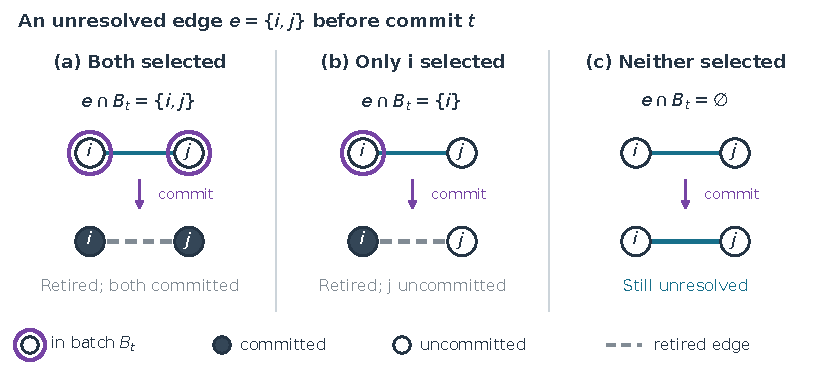
\includegraphics[width=\linewidth]{figures/c45_readability_2026-09-22/output/pdf/commit_cases.pdf}
 \caption{Three possible batch selections on an initially unresolved edge.
 Each panel shows the edge before (top) and after (bottom) one commit.
 Purple rings mark membership in $B_t$; filled nodes are committed.
 Selecting both endpoints gives a collision; selecting one gives a crossing
 edge. Both events retire the whole edge, but in (b) $j$ remains uncommitted.
 Selecting neither endpoint leaves the edge unresolved. The proof records
 the edge identity and both triggers in (a)--(b); the target matching itself
 is unchanged.}
 \label{fig:c4-matching-states}
\end{figure}


% Please keep this introduction with the first component-law definitions.
\Needspace{7\baselineskip}
\emph{Factor the two batch laws.}
Fix a compatible instance \(I\) and visible history \(h\), and write
\(B_t=B_t(h)\). Recall the committed set \(G(h)\), its values \(x_{G(h)}\),
and commit state \(y_t(h)\) from \cref{app:lower-proof-midpoint}.
For each edge \(e\in\HiddenMatching\), define two masses on
\(\Vocab^{e\cap B_t}\):
\begin{align*}
 p_e(z_{e\cap B_t})
 &:=\HardEdgeLaw{e}{I}\!\left(
   X_{e\cap B_t}=z_{e\cap B_t}
   \,\middle|\,
   X_{e\cap G(h)}=x_{e\cap G(h)}
 \right),\\
 \widehat p_e(z_{e\cap B_t})
 &:=\prod_{j\in e\cap B_t}
       \HardOracleRowMass{I}{y_t(h)}{j}{z_j}.
\end{align*}
The first is a conditional mass. The second is normalized because its
coordinates are distinct:
\[
 \sum_{z_{e\cap B_t}}p_e(z_{e\cap B_t})=1,
 \qquad
 \sum_{z_{e\cap B_t}}\widehat p_e(z_{e\cap B_t})
 =\prod_{j\in e\cap B_t}
   \left[\sum_{z_j\in\Vocab}
          \HardOracleRowMass{I}{y_t(h)}{j}{z_j}\right]=1.
\]
If \(e\cap B_t=\varnothing\), the space has one empty assignment and
both masses equal one there.

The sets \(e\cap B_t\) partition \(B_t\).
The edgewise product target law and the oracle product rule give
\begin{align*}
 \HardExactBatchLaw{t}{I}(z\mid h)
 &=\frac{\displaystyle\prod_{e\in\HiddenMatching}
      \HardEdgeLaw{e}{I}
       (X_{e\cap B_t}=z_{e\cap B_t},\,
        X_{e\cap G(h)}=x_{e\cap G(h)})}
     {\displaystyle\prod_{e\in\HiddenMatching}
      \HardEdgeLaw{e}{I}
       (X_{e\cap G(h)}=x_{e\cap G(h)})}\\
 &=\prod_{e\in\HiddenMatching}p_e(z_{e\cap B_t}),\\
 \HardProductBatchLaw{t}{I}(z\mid h)
 &=\prod_{j\in B_t}\HardOracleRowMass{I}{y_t(h)}{j}{z_j}
 =\prod_{e\in\HiddenMatching}\widehat p_e(z_{e\cap B_t}).
\end{align*}
Strict positivity makes every conditioning denominator positive.
These are products at fixed \(I,h\), before averaging over the instance.
Consequently,
\begin{equation}
 \sqrt{\HardExactBatchLaw{t}{I}(z\mid h)
       \HardProductBatchLaw{t}{I}(z\mid h)}
 =\prod_{e\in\HiddenMatching}
       \sqrt{p_e(z_{e\cap B_t})\widehat p_e(z_{e\cap B_t})}.
 \label{app:eq:commit-midpoint-numerator-factorization}
\end{equation}

\emph{Normalize edge by edge.}
Summing the preceding product over the disjoint coordinate blocks gives
\begin{align}
 \HardLocalAffinity{t}{I,h}
 &=\sum_{z\in\Vocab^{B_t}}
     \prod_{e\in\HiddenMatching}
       \sqrt{p_e(z_{e\cap B_t})\widehat p_e(z_{e\cap B_t})}\notag\\
 &=\prod_{e\in\HiddenMatching}
     \left[\sum_{u\in\Vocab^{e\cap B_t}}
                 \sqrt{p_e(u)\widehat p_e(u)}\right]\notag\\
 &=\prod_{e\in\HiddenMatching}\HellingerAffinity(p_e,\widehat p_e).
 \label{app:eq:local-affinity-survivor-factorization}
\end{align}
This is the product-affinity identity of
\cref{app:lem:finite-hellinger-calculus}, with index set
\(J=\HiddenMatching\), spaces \(\mathcal X_e=\Vocab^{e\cap B_t}\),
and the two component masses defined above.
Dividing the numerator product by this positive normalizing product yields
\begin{equation}
 \HardMidpointKernel{t}{I}(z\mid h)
 =\prod_{e\in\HiddenMatching}
 \frac{\sqrt{p_e(z_{e\cap B_t})\widehat p_e(z_{e\cap B_t})}}
      {\displaystyle\sum_{u\in\Vocab^{e\cap B_t}}
                 \sqrt{p_e(u)\widehat p_e(u)}}.
 \label{app:eq:normalized-commit-survivor-likelihood}
\end{equation}
Each factor is normalized: its sum over its coordinate block is its
denominator divided by itself, hence one. On an empty block, both numerator
and denominator are one.

At the fixed observed value \(z\), the factors have the following
dependencies:
\begin{center}
\small
\begin{tabularx}{\linewidth}{@{}>{\raggedright\arraybackslash}p{.23\linewidth}
 >{\raggedright\arraybackslash}X@{}}
\toprule
Edge status & What determines its normalized factor? \\
\midrule
Retired earlier
& Its identity and both triggers, the committed values, and the selected
batch are already in \(\OpAnalyticField{s}\). \\
\addlinespace
Retired in this commit
& Its identity and both triggers are in \(\RetiredRecordValue\);
the remaining inputs are in the current history. \\
\addlinespace
Still unresolved
& It misses \(B_t\), so \(e\cap B_t=\varnothing\) and its factor is \(1\),
for every possible edge identity and trigger assignment. \\
\bottomrule
\end{tabularx}
\end{center}
Thus the normalized kernel is unchanged when the survivor configuration
changes. The exact value of a collision's affinity is needed later in
\cref{app:lem:collision-affinity}; here only this independence is needed.

\emph{Include the oracle replies and identify the support.}
On an unresolved edge, both endpoints are still masked in \(y_t(h)\),
so every commit row there is \(\HardMarginal\).
Rows on earlier retired edges are determined by their recorded identities
and triggers, through \eqref{app:eq:hard-oracle}.
Hence the whole commit-row tuple is fixed by \(\OpAnalyticField{s}\).
For a compatible observation \(o=(\mathbf q,z)\),
\begin{align*}
 \OpSurvivorLikelihood{s}{(\mathbf q,z)}{\SurvivorConfigA}{\RetiredRecordValue}
 &=\mathbf 1\!\left\{
      \mathbf q=(\HardOracleRow{I}{y_t(h)}{j})_{j\in B_t}
    \right\}
    \HardMidpointKernel{t}{I}(z\mid h)\\
 &=\HardMidpointKernel{t}{I}(z\mid h)>0.
\end{align*}
The fixed old and new retirement records, together with
\(\SurvivorConfigA\), specify \(I\). The table shows that the resulting
likelihood has the same positive value for every compatible
\(\SurvivorConfigA\).

Every previously unresolved edge touching \(B_t\) is in
\(\RetiredRecordValue\). Thus
\(\OpUnresolvedVertices{s+1}\cap B_t=\varnothing\), and no surviving
candidate is tested by this commit. The full support is
\[
 \operatorname{PM}(\OpUnresolvedVertices{s+1})
 \times\prod_{i\in\OpUnresolvedVertices{s+1}}\OpRemainingTriggers{i}{s},
 \qquad
 \OpRemainingTriggers{i}{s+1}=\OpRemainingTriggers{i}{s}
 \quad(i\in\OpUnresolvedVertices{s+1}).
\]
Indeed, each configuration in this product extends uniquely with the
retired record, produces the same oracle rows, and assigns positive
midpoint probability to the observed batch value.
It retires exactly the same edges because the surviving vertices
are disjoint from \(B_t\).

\emph{5. Normalize the posterior and conclude (IH\(_{s+1}\)).}
Steps 3--4 give the full support
\[
 \mathcal Z_{s+1}:=
 \operatorname{PM}(\OpUnresolvedVertices{s+1})
 \times\prod_{i\in\OpUnresolvedVertices{s+1}}
                 \OpRemainingTriggers{i}{s+1}.
\]
Step~2 gives equal pre-observation weights, and the query or commit
calculation gives equal positive likelihoods on this support.
Consequently, for any \(\SurvivorConfigA\in\mathcal Z_{s+1}\), the
denominator in \eqref{app:eq:survivor-bayes-odds} is
\begin{align*}
 &\sum_{\mathfrak u\in\mathcal Z_{s+1}}
  \mathbb P(\OpSurvivorState{s+1}=\mathfrak u,
       \OpRetiredRecord{s}=\RetiredRecordValue\mid\OpAnalyticField{s})
       \OpSurvivorLikelihood{s}{o}{\mathfrak u}{\RetiredRecordValue}\\
 &\quad=|\mathcal Z_{s+1}|\,
  \mathbb P(\OpSurvivorState{s+1}=\SurvivorConfigA,
       \OpRetiredRecord{s}=\RetiredRecordValue\mid\OpAnalyticField{s})
       \OpSurvivorLikelihood{s}{o}{\SurvivorConfigA}{\RetiredRecordValue}.
\end{align*}
The common numerator is positive, so cancellation yields
\[
 \mathbb P(\OpSurvivorState{s+1}=\SurvivorConfigA
                 \mid\OpAnalyticField{(s+1)})
 =\frac1{|\mathcal Z_{s+1}|}
 =\frac1{|\operatorname{PM}(\OpUnresolvedVertices{s+1})|}
     \prod_{i\in\OpUnresolvedVertices{s+1}}
       \frac1{|\OpRemainingTriggers{i}{s+1}|}.
\]
This is the independent product required by (IH\(_{s+1}\)).
Induction proves the law at every operation boundary, including the
terminal boundary after the last operation.  There the unresolved set is
empty and the law is the point mass on the empty state.
Finally, the event that operation \(s\) is commit \(t\) is already known
at that operation's starting boundary:
\[
 \{s_t=s\}
 =\left\{\sum_{r<s}\mathbf 1\{A_r\text{ is a commit}\}=t-1,
             \ A_s\text{ is a commit}\right\}
 \in\OpAnalyticField{s}.
\]
Apply (IH\(_s\)) on each of these events to obtain the law at the
adaptive boundary \(s_t\).  At that boundary,
\(\OpSurvivorState{s_t}=\SurvivorState{t}\) and
\(\OpAnalyticField{s_t}=\AnalyticField{t}\), hence
\eqref{app:eq:strong-survivor-invariant} at every pre-commit boundary.
\end{proof}
\fi

% This figure is also used by the subsequent edge-counting argument, so it
% remains compiled even though the legacy proof containing its old call site
% is retained only as noncompiled source.
% Please show each local selection pattern at manuscript width, without a full-page float.
\begin{figure}[!htbp]
 \centering
 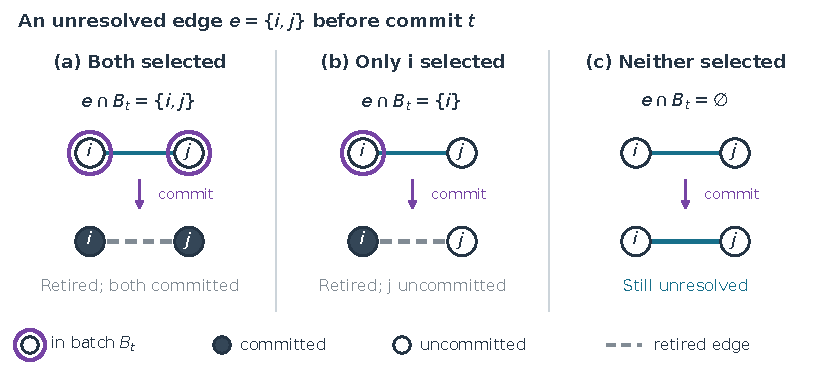
\includegraphics[width=\linewidth]{figures/c45_readability_2026-09-22/output/pdf/commit_cases.pdf}
 \caption{Three possible batch selections on an initially unresolved edge.
 Each panel shows the edge before (top) and after (bottom) one commit.
 Purple rings mark membership in $B_t$; filled nodes are committed.
 Selecting both endpoints gives a collision; selecting one gives a crossing
 edge. Both events retire the whole edge, but in (b) $j$ remains uncommitted.
 Selecting neither endpoint leaves the edge unresolved. The proof records
 the edge identity and both triggers in (a)--(b); the target matching itself
 is unchanged.}
 \label{fig:c4-matching-states}
\end{figure}


\paragraph{One source, at most one candidate per submission.}
Recall from \cref{app:eq:unresolved-matching-update,app:eq:retirement-record}
that the number of query-retired edges is
\[
 \GenieDeletions
 =\sum_{s:\,A_s\text{ is a query}}
   |\OpUnresolvedMatching{s}\setminus\OpUnresolvedMatching{s+1}|.
\]
Commit retirements do not contribute, and simultaneous hits at both endpoints
count as one edge.
A state \(y\) tests at most one candidate \(\HardTest{y}{i}\) at each source
\(i\), regardless of how many returned rows are inspected.
Together with the conditional uniformity in
\cref{app:lem:unresolved-invariant}, this gives the following bound directly.

\begin{lemma}[Equality-test disclosure]
\label{app:lem:query-disclosure}
For any algorithm using at most \(\QueryBudget{}\) counterfactual submissions,
\begin{equation}
 \mathbb E\GenieDeletions\le\frac{N\QueryBudget{}}{\HardBankSize}.
 \label{app:eq:expected-query-deletions}
\end{equation}
\end{lemma}

\begin{proof}
All probabilities and expectations use the joint instance--midpoint law
\eqref{app:eq:joint-instance-midpoint-law}, with the decision-rule seed
\(w\) fixed. The execution below is the midpoint execution.
It suffices to consider integer \(\QueryBudget{}\): for a noninteger
budget, apply the integer result to \(\lfloor\QueryBudget{}\rfloor\),
whose bound is no larger.
If \(\QueryBudget{}=0\), there are no query hits and
\(\GenieDeletions=0\). If \(\QueryBudget{}\ge\HardBankSize\), the bound
follows from \(\GenieDeletions\le N/2\le N\QueryBudget{}/\HardBankSize\).
Hence assume \(1\le\QueryBudget{}<\HardBankSize\).

\emph{1. Bound the hit probability at one query.}
Fix a vertex \(i\). Number counted counterfactual submissions by
\(k=1,2,\ldots\); commits may occur between them.
The distinguished all-mask preprocessing readout tests no candidate
and is not included in this count.
At the \(k\)-th such query, let \(s\) be its operation index and write
\(y=\OpSubmittedState{s}\), as in \cref{app:eq:operation-action}.
Recall that
\(\OpUnresolvedVertices{s}=\bigcup_{e\in\OpUnresolvedMatching{s}}e\)
is the unresolved vertex set just before this operation
(\cref{app:eq:unresolved-vertices}).
The past and selected action determine whether operation \(s\) is
the \(k\)-th counted query. Thus the operation-boundary conclusion of
\cref{app:lem:unresolved-invariant} applies here even when the query
time and state are chosen adaptively.

If \(i\in\OpUnresolvedVertices{s}\), each of the preceding \(k-1\)
counted submissions has removed at most one candidate at \(i\).
Commits leave the candidate set of a surviving vertex unchanged, by
\cref{app:eq:operation-candidates}. Consequently,
\[
 |\OpRemainingTriggers{i}{s}|
 \ge \HardBankSize-(k-1)=\HardBankSize-k+1.
\]
Conditional on \(\OpAnalyticField{s}\), the submitted state is fixed
and \(\TriggerIndex{i}\) is uniform on
\(\OpRemainingTriggers{i}{s}\). Therefore
\begin{align}
 \mathbb P(\HardHit{y}{i}=1\mid\OpAnalyticField{s})
 &=\mathbb P(\TriggerIndex{i}=\HardTest{y}{i}
                  \mid\OpAnalyticField{s})\notag\\
 &=\frac{\mathbf 1\{\HardTest{y}{i}\in\OpRemainingTriggers{i}{s}\}}
         {|\OpRemainingTriggers{i}{s}|}
 \le\frac1{\HardBankSize-k+1}.
 \label{app:eq:query-conditional-hit-bound}
\end{align}
A mask, background token, or previously excluded candidate gives numerator
zero. If the edge has already retired, there can be no further hit
\emph{while unresolved}, regardless of later oracle replies.

\emph{2. Accumulate the probabilities without assuming independence.}
For \(0\le k\le\QueryBudget{}\), define
\[
 p_{i,k}:=
 \mathbb P\!\left(
 \begin{gathered}
 i\text{ has a query hit while its edge is unresolved}\\
 \text{among the first }k\text{ counted submissions}
 \end{gathered}
 \right),
 \qquad p_{i,0}=0.
\]
If the execution contains fewer than \(k\) counted submissions, this event
uses all those that occurred; no extra queries are executed.
A hit retires the edge, so \(i\) can have at most one hit while unresolved.
The increment \(p_{i,k}-p_{i,k-1}\) is therefore the probability of such
a hit at query \(k\).

To bound this increment, condition on each possible analytic history
just before query \(k\), apply
\eqref{app:eq:query-conditional-hit-bound} when \(i\) is unresolved,
and average over these histories. This gives
\begin{align}
 p_{i,k}-p_{i,k-1}
 &\le
 \frac{\mathbb P(\text{query }k\text{ occurs and }i
                  \text{ is unresolved just before it})}
      {\HardBankSize-k+1}\notag\\
 &\le\frac{1-p_{i,k-1}}{\HardBankSize-k+1}.
 \label{app:eq:query-hit-recurrence}
\end{align}
For the last inequality, an unresolved vertex has not hit earlier.
Earlier retirement by a mate hit or a commit, as well as early termination,
can only remove paths from the event in the numerator.
Simultaneous hits at \(i\) and its mate still count as a hit at \(i\):
the edge was unresolved immediately before that query.

Rearranging \eqref{app:eq:query-hit-recurrence} step by step yields
\begin{align*}
 1-p_{i,k}
 &=1-p_{i,k-1}-(p_{i,k}-p_{i,k-1})\\
 &\ge(1-p_{i,k-1})
       \left(1-\frac1{\HardBankSize-k+1}\right)\\
 &=(1-p_{i,k-1})
       \frac{\HardBankSize-k}{\HardBankSize-k+1}.
\end{align*}
Starting from \(1-p_{i,0}=1\) and applying this inequality successively,
\begin{align*}
 1-p_{i,\QueryBudget{}}
 &\ge
 \prod_{k=1}^{\QueryBudget{}}
       \frac{\HardBankSize-k}{\HardBankSize-k+1}\\
 &=\frac{\HardBankSize-1}{\HardBankSize}
   \frac{\HardBankSize-2}{\HardBankSize-1}\cdots
   \frac{\HardBankSize-\QueryBudget{}}
        {\HardBankSize-\QueryBudget{}+1}\\
 &=\frac{\HardBankSize-\QueryBudget{}}{\HardBankSize}.
\end{align*}
For \(\QueryBudget{}=1\) the product has just its first factor.
The cancellation therefore gives
\begin{equation}
 p_{i,\QueryBudget{}}
 \le 1-\frac{\HardBankSize-\QueryBudget{}}{\HardBankSize}
 =\frac{\QueryBudget{}}{\HardBankSize}.
 \label{app:eq:query-source-hit-bound}
\end{equation}
This multiplication iterates conditional probability bounds; it does not
assume independent queries.

\emph{3. Count retired edges by their successful endpoints.}
At a query, an unresolved edge retires exactly when at least one of its
endpoints hits. For binary bits \(b_u,b_v\),
\(\mathbf 1\{b_u+b_v\ge1\}\le b_u+b_v\); two simultaneous hits still retire
only one edge. Hence, pathwise,
\[
 \begin{aligned}
 \GenieDeletions
 &=\sum_{s:\,A_s\text{ is a query}}
   \sum_{\{u,v\}\in\OpUnresolvedMatching{s}}
   \mathbf 1\{\HardHit{\OpSubmittedState{s}}{u}
              +\HardHit{\OpSubmittedState{s}}{v}\ge1\}\\
 &\le
   \sum_{i=1}^N
   \sum_{\substack{s:\,A_s\text{ is a query}\\
                    i\in\OpUnresolvedVertices{s}}}
             \HardHit{\OpSubmittedState{s}}{i}.
 \end{aligned}
\]
The change from edges to vertices uses that every unresolved vertex lies
on exactly one matching edge.
For each \(i\), the inner sum is either zero or one, because its first
hit retires its edge. It is thus the indicator of the event defining
\(p_{i,\QueryBudget{}}\). Taking expectations and using
\(\mathbb E\mathbf 1_E=\mathbb P(E)\) gives
\[
 \begin{aligned}
 \mathbb E\GenieDeletions
 &\le
 \sum_{i=1}^N\mathbb E\!\left[
   \sum_{\substack{s:\,A_s\text{ is a query}\\
                    i\in\OpUnresolvedVertices{s}}}
             \HardHit{\OpSubmittedState{s}}{i}\right]\\
 &=\sum_{i=1}^N p_{i,\QueryBudget{}}
 \le\sum_{i=1}^N\frac{\QueryBudget{}}{\HardBankSize}
 =\frac{N\QueryBudget{}}{\HardBankSize}.
 \end{aligned}
\]
No independence between vertices is used.
\end{proof}
\FloatBarrier
